\documentclass[8pt]{beamer}

\usepackage{polski}
\usepackage[utf8]{inputenc}
\usepackage[T1]{fontenc}
\usepackage[polish]{babel}
\usepackage{lmodern}
\usepackage{mathptmx}
\usepackage{amsmath}
\usepackage{color}
\usepackage[normalem]{ulem}
\usepackage{graphicx}
\usepackage{hyperref}
\usepackage{listings}

\hypersetup{
  colorlinks
}

\pdfcompresslevel 9
\pdfobjcompresslevel 9

\lstset{
  language=c,
  basicstyle=\small\ttfamily,
  keywordstyle=\color{blue}\ttfamily,
  stringstyle=\color{red}\ttfamily,
  directivestyle=\color{magenta}\ttfamily,
  commentstyle=\color{darkgray}\ttfamily,
  numberstyle=\color{gray}\tiny,
  numbersep=-15pt,
  extendedchars=true
}

\mode<beamer>
{
  \usetheme{Frankfurt}
  \useoutertheme{miniframes}
  \setbeamercovered{transparent}
}

\subject{Talks}

\pgfdeclareimage[height=10mm]{university-logo}{images/logo}
\logo{\pgfuseimage{university-logo}}

\AtBeginSection[]
{
  \begin{frame}<beamer>{}
    \tableofcontents[currentsection]
  \end{frame}
}

\title{Systemy wbudowane}
\subtitle{Arduino: Programowanie niskopoziomowe}
\author[Krystian Bacławski]{\href{mailto:cahirwpz@cs.uni.wroc.pl}{Krystian Bacławski}}
\institute[Instytut Informatyki]{Uniwersytet Wrocławski}
\date{\today}

\begin{document}

\begin{frame}
  \titlepage
\end{frame}

\begin{frame}
  \begin{enumerate}
    \item Programowanie bez Arduino IDE.
    \item Elementy programowania układu \texttt{Atmega 328P}.
  \end{enumerate}
\end{frame}

\section*{Programowanie bez Arduino IDE}

\begin{frame}[fragile]
  \frametitle{Kompilacja i szkielet pliku Makefile}

  \begin{exampleblock}{}
    \begin{lstlisting}[language=make,numbers=left]
      MCU    = atmega328p
      CC     = avr-gcc -mmcu=$(MCU)
      CFLAGS = -O2 -Wall -Wextra
      PORT   = $(wildcard /dev/tty.usbmodemf*)

      all: program.hex

      program.elf: program.o uart.o
      usart.o: usart.c usart.h

      %.elf: %.o
        $(CC) $(CFLAGS) -o $@ $^

      %.hex: %.elf
        avr-objcopy -j .text -j .data -O ihex $< $@

      install: $(PRG).hex
        avrdude -p $(MCU) -c arduino -P $(PORT) \
          -v -U flash:w:$(PRG).hex 

      clean:
        @rm -vf *.{elf,hex,o,map} *~
    \end{lstlisting}
  \end{exampleblock}
\end{frame}

\begin{frame}[fragile]
  \frametitle{Model pamięci i sekcje programu}
  Polecenie \verb#avr-objdump -h section.elf# pokazuje, że są tylko 3 sekcje:
  \begin{description}
    \item[.text] kodu i stałych w pamięci programu.
    \item[.data] danych zarówno zmiennych i stałych (normalnie \texttt{.rodata})
    \item[.bss] danych niezainicjalizowanych
  \end{description}

  \begin{alertblock}{}
    Procesory AVR realizują \href{http://en.wikipedia.org/wiki/Harvard_architecture}{architekturę harvardzką}!
    Pamięć programu (\texttt{FLASH}), pamięć nieulotna (\texttt{EEPROM}),
    pamięć danych (\texttt{RAM}) i szyna urządzeń \texttt{IO} są rozłączne!
    Biblioteka standardowa oferuje klony funkcji działające na pamięci programu
    (sufiks \verb#_P#).
  \end{alertblock}

  \begin{exampleblock}{}
    \begin{lstlisting}[numbers=left]
      #include <avr/pgmspace.h>

      const int ro_int = 10;
      const int ro_arr[5] = { 10, 20, 30, 40, 50 };
      const int arr[5] PROGMEM = { 1, 2, 3, 4, 5 };

      int rw_int = 20;
      int rw_arr_bss[10];
      int rw_arr[5] = { 32, 64, 128, 256, 512 };
    \end{lstlisting}
  \end{exampleblock}
\end{frame}

\begin{frame}[fragile]
  \frametitle{Rozkład pamięci, a inicjalizacja programu}

  \begin{alertblock}{}
    Kod w sekcji \texttt{.initN} dla $N = {0..9}$ wykonuje się przed wejściem do funkcji
    \texttt{main()}.
    \begin{description}
      \item[.init2] inicjalizuje wskaźnik stosu i zeruje stos.
      \item[.init4] kopiuje \texttt{.data} do pamięci \texttt{RAM}, oraz
        zapisuje sekcję \texttt{BSS} zerami. 
    \end{description}
  \end{alertblock}

  \begin{center}
    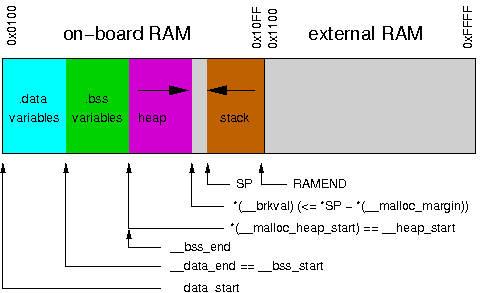
\includegraphics[scale=0.5]{images/malloc-std.png}
  \end{center}
\end{frame}

\begin{frame}[fragile]
  \frametitle{Przerwania}

  \begin{lstlisting}[language=c]
    #include <avr/interrupt.h>

    ISR(ADC_vect) {
      ...
    }

    /* for undefined interrupts */
    ISR(BADISR_vect) {
      ...
    }

    /* for nested interrupts */
    ISR(XXX_vect, ISR_NOBLOCK)
    {
      ...
    }

    /* using same handler for two interrupts */
    ISR(PCINT0_vect) {
      ...
    }

    ISR(PCINT1_vect, ISR_ALIASOF(PCINT0_vect));
  \end{lstlisting}
\end{frame}

\begin{frame}[fragile]
  \frametitle{Komunikacja z Arduino}

  Można korzystać z pythonowej biblioteki \href{http://pyserial.sourceforge.net/}{pySerial}.

  \begin{exampleblock}{Terminal szeregowy}
    \begin{lstlisting}[language=sh,gobble=5]
      #!/bin/sh

      PORT=$(ls -1 /dev/tty.usbmodemf*)
      BAUD=38400

      python -m serial.tools.miniterm $PORT $BAUD
    \end{lstlisting}
  \end{exampleblock}

  \begin{exampleblock}{Skryptowanie komunikacji}
    \begin{lstlisting}[language=python,gobble=5]
      import serial

      ser = serial.Serial(0)  # open first serial port
      print ser.name          # check which port was really used
      ser.write("hello")      # write a string
      s = ser.read(10)        # read up to ten bytes (timeout)
      line = ser.readline()   # read a '\n' terminated line
      ser.close()             # close port
    \end{lstlisting}
  \end{exampleblock}
\end{frame}

\section*{Elementy programowania układu \texttt{Atmega 328P}}

\begin{frame}
  \frametitle{Schemat blokowy mikrokontrolera}

  \begin{center}
    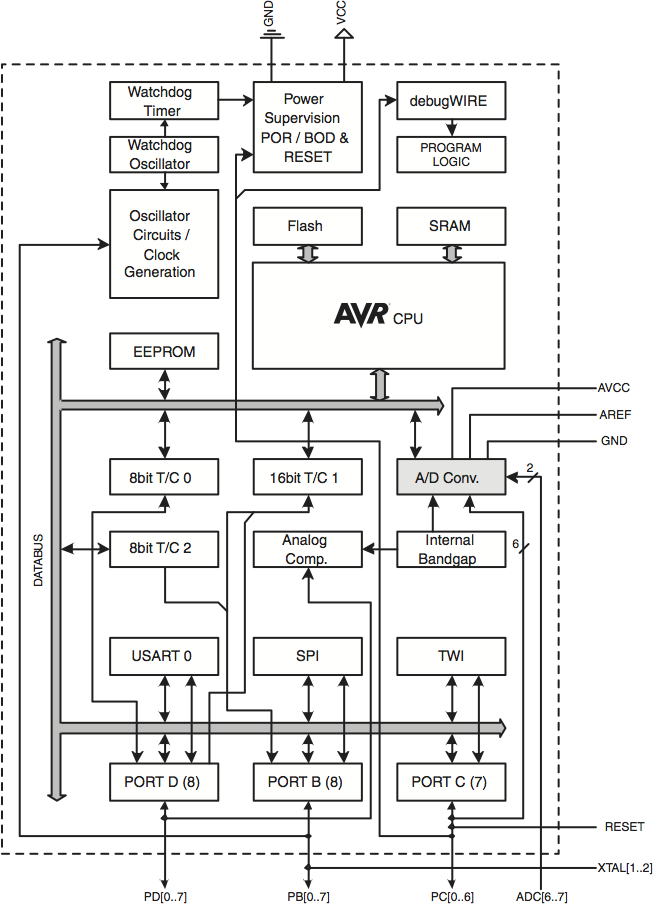
\includegraphics[scale=0.5]{images/atmega328p.png}
  \end{center}
\end{frame}

\begin{frame}
  \frametitle{Zegar systemowy.}

  \begin{itemize}
    \item Funkcje \texttt{clock\_prescale\_set} i \texttt{clock\_prescale\_get}
      służą do zmiany częstotliwości taktowania w trakcie działania programu.
    \item Programowanie \texttt{EEPROM} i \texttt{FLASH} nakłada ścisłe
      ograniczenia na czas.
    \item Watchdog resetuje mikrokontroler, jeśli program nie zapisze rejestru
      co jakiś ustalony czas -- metoda wykrywania zawieszeń. Nagłówek \texttt{<avr/wdt.h>}.
  \end{itemize}

  \begin{center}
    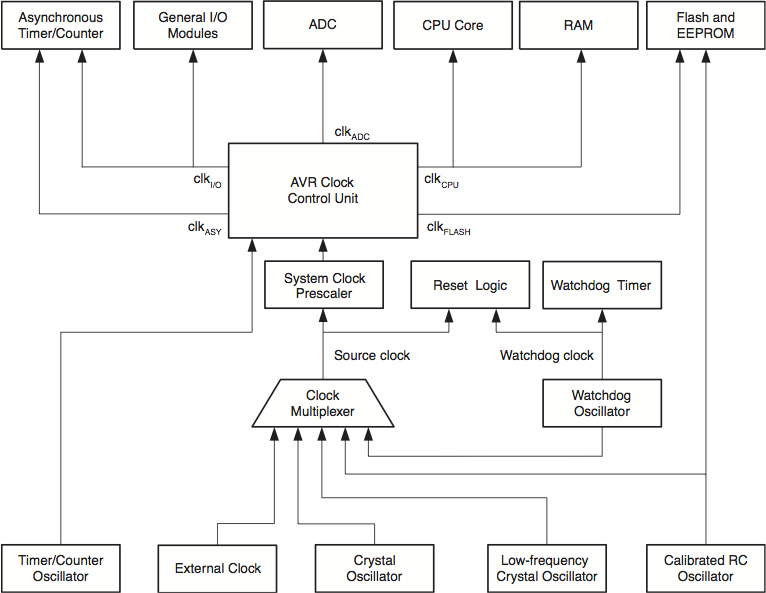
\includegraphics[scale=0.5]{images/clock.png}
  \end{center}
\end{frame}

\begin{frame}
  \frametitle{Zarządzanie energią}

  \begin{block}{}
    Nagłówek \texttt{<avr/power.h>} oferuje włączanie i wyłączanie
    poszczególnych podsystemów mikrokontrolera -- np.: czasomierze, konwerter
    analogowo-cyfrowy, itd.
  \end{block}

  \begin{block}{}
    Nagłówek \texttt{<avr/sleep.h>} umożliwia usypianie procesora i jego
    podsystemów. Szybkość wybudzania jest uzależniona źródłem taktowania
    procesora.
  \end{block}

  \begin{exampleblock}{Poziomy uśpienia.}
    W zależności od poziomu, procesor może być wybudzony różnymi zdarzeniami:

    \begin{itemize}
      \item koniec konwersji analogowo-cyfrowej, zapisu do \texttt{EEPROM},
      \item transmisji \texttt{UART} / \texttt{SPI} / \texttt{TWI},
      \item przerwanie czasomierza lub zewnętrzne (\texttt{INT0}, \texttt{INT1}),
      \item odebranie pakietu o adresie odpowiadającym mikrokontrolerowi (\texttt{TWI}).
    \end{itemize}

    \ldots oczywiście pod warunkiem, że źródła zdarzeń zostały odpowiednio
    skonfigurowane.
  \end{exampleblock}
\end{frame}

\begin{frame}
  \frametitle{Przerwania}

  \begin{columns}
    \begin{column}{8cm}
      \begin{center}
        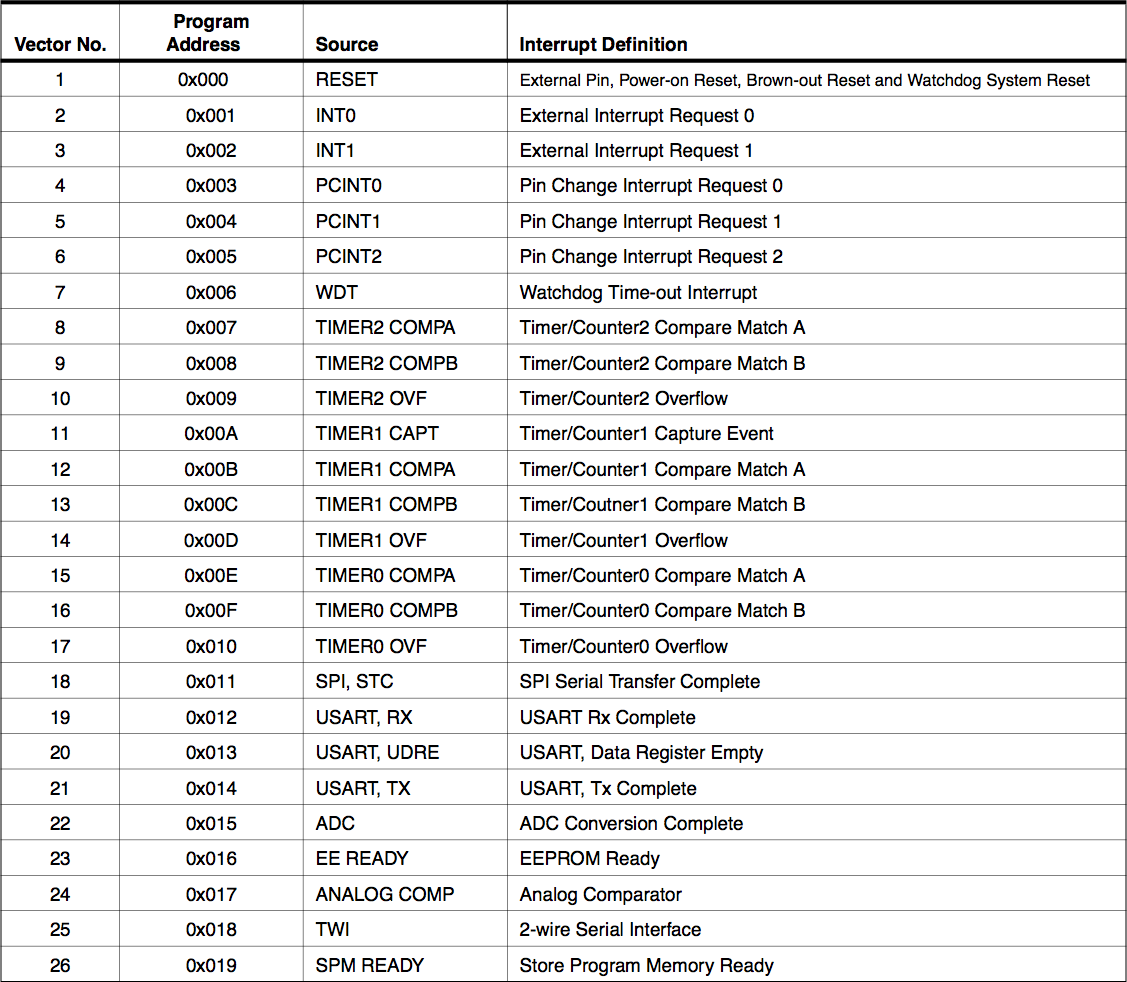
\includegraphics[scale=0.4]{images/interrupts.png}
      \end{center}
    \end{column}
    
    \begin{column}{2.5cm}
      Odpalane o ile dany podsystem został odpowiednio skonfigurowany.

      \vspace{1em}

      Wstrzymanie lub wznowienie obsługi przerwań przy pomocy instrukcji
      \texttt{sei} i \texttt{cli}.

      \vspace{1em}

      Przerwania wyzwalane stanem pinów podpięte pod wektory \texttt{PCINTn}.
      Konretny numer pinu w specjalnym rejestrze.
    \end{column}
  \end{columns}
\end{frame}

\begin{frame}
  \frametitle{Konfiguracja portów}

  \begin{block}{}
    Nagłówek \texttt{<avr/io.h>} zawiera definicje wszystkich rejestrów
    \texttt{IO} procesorów \texttt{AVR}.

    \vspace{1em}

    Dla każdego portu istnieją trzy rejestry:
    \begin{description}
      \item[\texttt{DDRn}] konfiguracja kierunku portów (wejście / wyjście),
      \item[\texttt{PORTn}] wartość portów wyjściowych,
      \item[\texttt{PINn}] wartość portów wejściowych.
    \end{description}
  \end{block}

  \begin{block}{}
    Nagłówek \texttt{<avr/sfr\_defs.h>} oferuje kilka użytecznych makr:
    \begin{itemize}
      \item \texttt{\_BV(BIT)},
      \item \texttt{loop\_until\_bit\_is\_clear(REG, BIT)},
      \item \texttt{bit\_is\_set(REG, BIT)}, ...
    \end{itemize}
  \end{block}

  \begin{block}{Porty, a piny Arduino:}
    \begin{itemize}
      \item $PD0..PD7$ $\rightarrow$ $0..7$,
      \item $PB0..PB5$ $\rightarrow$ $8..13$,
      \item $PC0..PC5$ $\rightarrow$ $A0..A5$.
    \end{itemize}
  \end{block}
\end{frame}

\begin{frame}
  \frametitle{Alternatywne funkcje portów}

  \begin{columns}
    \begin{column}[T]{5cm}
      \begin{center}
        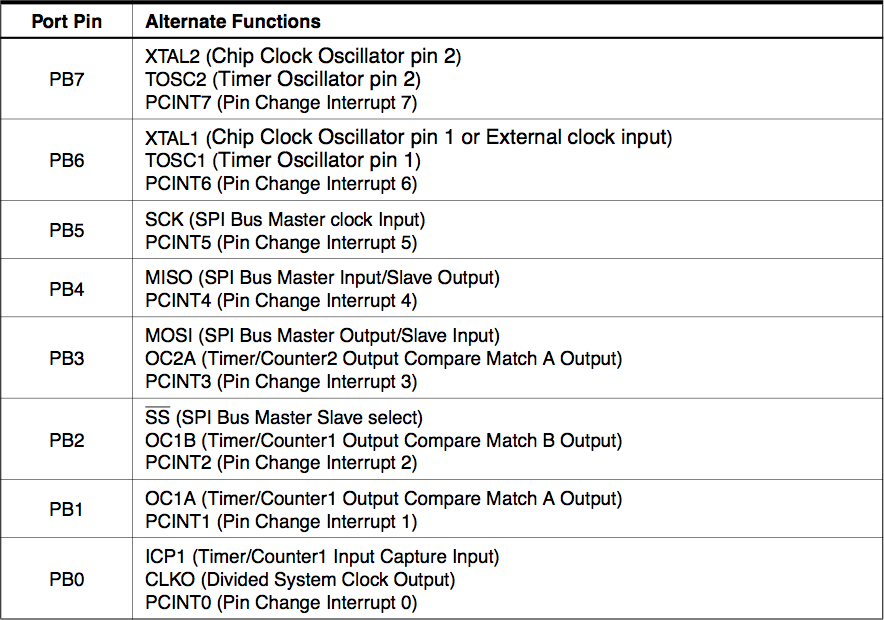
\includegraphics[scale=0.3333]{images/port-b.png}
      \end{center}
      \begin{center}
        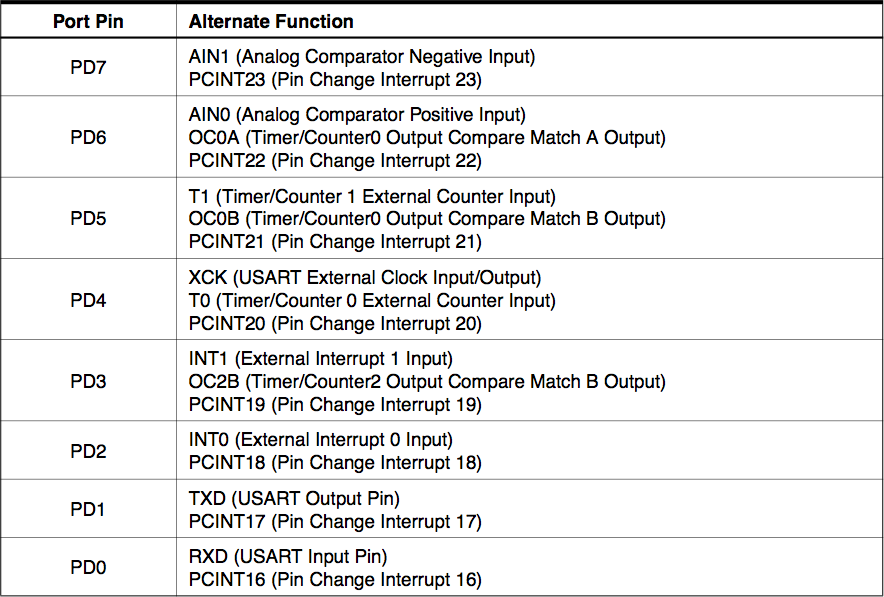
\includegraphics[scale=0.3333]{images/port-d.png}
      \end{center}
    \end{column}
    
    \begin{column}[T]{5.5cm}
      \begin{center}
        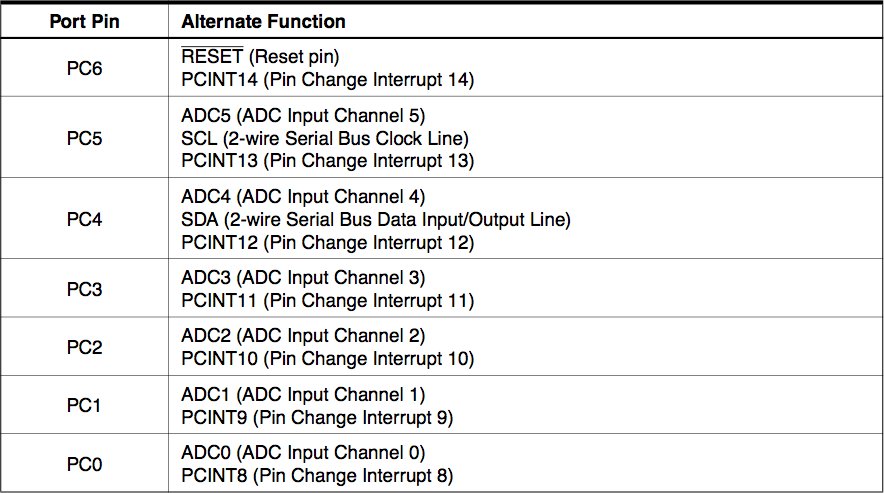
\includegraphics[scale=0.3333]{images/port-c.png}
      \end{center}

      W zależności od konfiguracji podsystemów porty nabierają innego
      znaczenia. Czasami jest istotne czy skonfigurujemy je jako wejście czy
      wyjście zanim zaczniemy korzystać z alternatywnej funkcji.

    \end{column}
  \end{columns}
\end{frame}

\begin{frame}
  \frametitle{Schemat blokowy czasomierza \texttt{Timer0}}

  Wszystkie dostarczają bardzo podobnej funkcjonalności. Liczniki i komparatory
  dla \texttt{Timer0} i \texttt{Timer2} są 8-bitowe, dla \texttt{Timer1}
  16-bitowe. Mogą sterować niektórymi podsystemami bez udziału procesora.
  Potrafią zgłaszać szereg różnych przerwań i generować fale prostokątne na
  wyjściach oznaczonych PWM (\textasciitilde). Różne tryby operacji
  (\texttt{normal}, \texttt{CTC}, \texttt{fast PWM}, \texttt{phase correct
    PWM}). W pełni konfigurowalne (dużo opcji).

  \begin{center}
    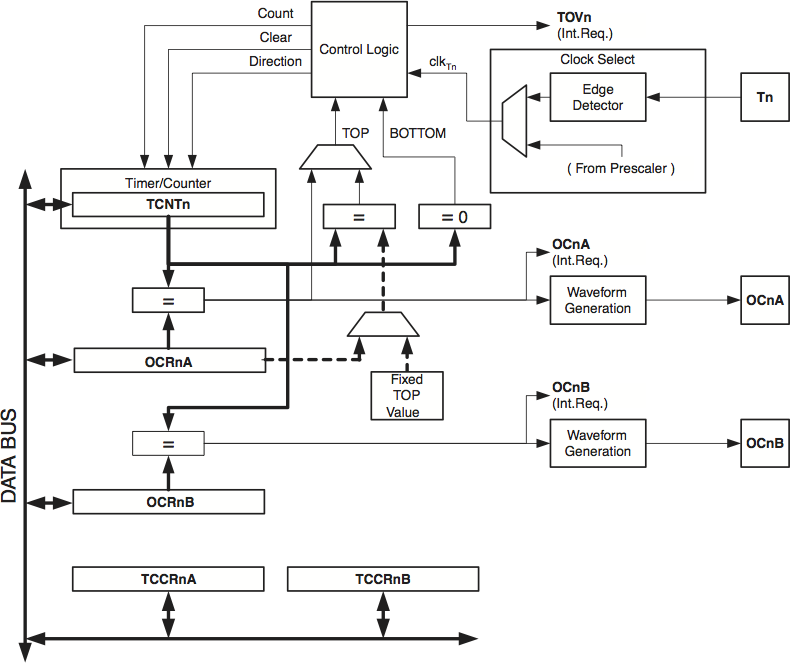
\includegraphics[scale=0.5]{images/timer.png}
  \end{center}
\end{frame}

\begin{frame}
  \frametitle{Generowanie fal prostokątnych z użyciem czasomierzy}

  Częstotliwość fali jest zadana wzorem $f_{clk_{I/O}} / (N \cdot 256)$, gdzie
  $N$ to wartość dzielnika częstotliwości $N \in \{1,8,64,256,1024\}$.  Jeśli
  porównanie \texttt{TCNTn} z rejestrem \texttt{OCRnA} zakończy się sukcesem,
  stan odpowiedniego pinu zostanie zmodyfikowany (\texttt{clear}, \texttt{set},
  \texttt{toggle}) i zostanie wygenerowane przerwanie. Można ustalić jaka
  wartość pinu zostanie ustalona przy przepełnieniu \texttt{TCNTn}.
  
  \begin{exampleblock}{}
    Używane przez \textit{Arduino IDE} do realizacji funkcji \texttt{analogWrite}.
  \end{exampleblock}

  \begin{center}
    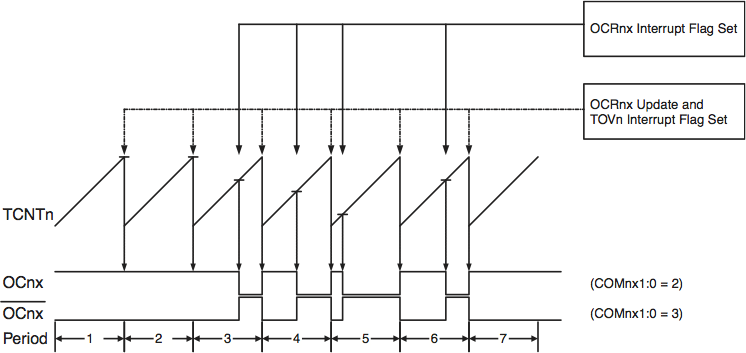
\includegraphics[scale=0.75]{images/fast-pwm.png}
  \end{center}
\end{frame}

\begin{frame}
  \frametitle{Konwerter cyfrowo-analogowy}

  Może być wysterowany z czasomierzy lub uruchamiany bezpośrednio.  Można
  mierzyć tylko jedną wartość na raz. Metoda pomiaru -- podział binarny. Czas
  pobierania próbki jest duży -- max. kilkadziesiąt tysięcy razy na sekundę w
  zależności od dokładności (8~lub 10 bit). Wymaga kalibracji -- pierwsza
  próbka do śmieci. Po zakończeniu może generować przerwanie i wybudzać procesor.

  \begin{center}
    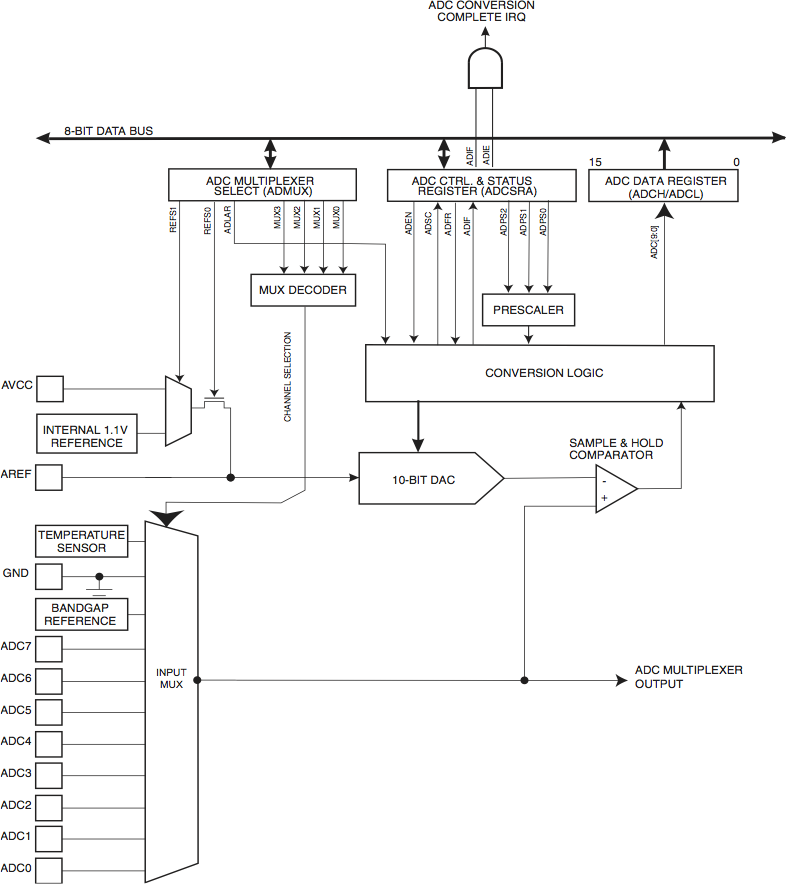
\includegraphics[scale=0.4]{images/adc.png}
  \end{center}
\end{frame}

\begin{frame}
  \frametitle{Interfejs SPI}

  SPI to szybki (do 8Mb/s) i prosty interfejs do komunikacji urządzeniami
  zewnętrznymi np.: wyświetlacze LCD, moduły radiowe, karty SDHC, przetworniki
  D/A, itd.

  \vspace{1em}

  Wszystkie urządzenia są połączone trzema drutami: \texttt{MISO} (Master-In
  Slave-Out), \texttt{MOSI} (Master-Out Slave-In) i \texttt{SCK} (System
  Clock). Poszczególne urządzenia wybieramy drutem \texttt{SS} (Slave Select).
  Dane są przepychane synchronicznie względem zegara, bit po bicie do
  wyczerpania bufora. Zakończenie transmisji może generować przerwanie.

  \begin{center}
    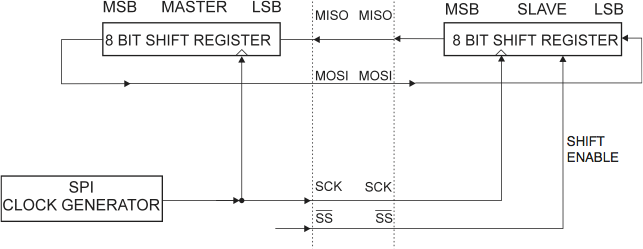
\includegraphics[scale=0.6666]{images/spi.png}
  \end{center}
 
  \begin{alertblock}{}
    Połączenie jest w pełni dupleksowe -- zawsze jednocześnie wysyłamy i
    odbieramy!
  \end{alertblock}

\end{frame}

%\begin{frame}
%  \frametitle{Interfejs USART}
%\end{frame}

%\begin{frame}
%  \frametitle{Interfejs TWI}
%\end{frame}

%\begin{frame}
%  \frametitle{Programowanie pamięci \texttt{EEPROM} i \texttt{FLASH}}
%\end{frame}

\end{document}
